\begin{tikzpicture}
  \node[inner sep=0pt, anchor=south west] (photo) at (0,0)
  {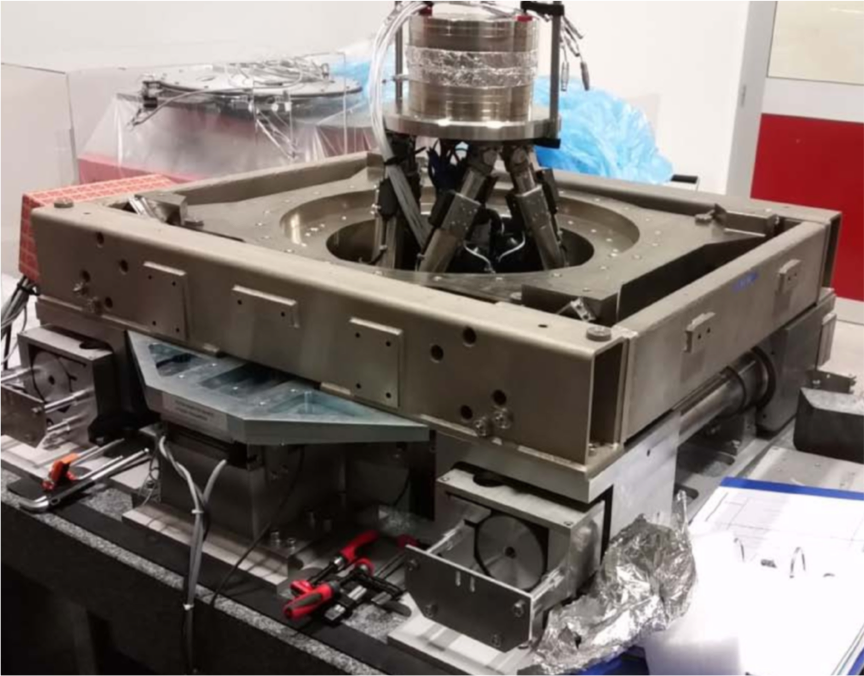
\includegraphics[width=0.39\textwidth]{/home/thomas/Cloud/thesis/papers/dehaeze18_sampl_stabil_for_tomog_exper/tikz/img/exp_setup_photo.png}};

  \coordinate[] (aheight) at (photo.north west);
  \coordinate[] (awidth)  at (photo.south east);

  \coordinate[] (granite) at ($0.1*(aheight)+0.1*(awidth)$);
  \coordinate[] (trans)   at ($0.5*(aheight)+0.4*(awidth)$);
  \coordinate[] (tilt)    at ($0.65*(aheight)+0.75*(awidth)$);
  \coordinate[] (hexapod) at ($0.7*(aheight)+0.5*(awidth)$);
  \coordinate[] (sample)  at ($0.9*(aheight)+0.55*(awidth)$);

  % Granite
  \node[labelc] at (granite) {1};
  % Translation stage
  \node[labelc] at (trans) {2};
  % Tilt Stage
  \node[labelc] at (tilt) {3};
  % Micro-Hexapod
  \node[labelc] at (hexapod) {4};
  % Sample
  \node[labelc] at (sample) {5};

  % Axis
  \begin{scope}[shift={($0.07*(aheight)+0.87*(awidth)$)}]
    \draw[->] (0, 0) -- ++(55:0.7) node[above] {$y$};
    \draw[->] (0, 0) -- ++(90:0.9) node[left] {$z$};
    \draw[->] (0, 0) -- ++(-20:0.7) node[above] {$x$};
  \end{scope}
\end{tikzpicture}
